\documentclass[12pt]{article}
\usepackage[margin=2.54cm]{geometry}

\usepackage{graphicx}
\usepackage[utf8]{inputenc}
\usepackage{csquotes}

\graphicspath{ {./imgs/} }

\usepackage[spanish]{babel}
\usepackage{hyperref}
\hypersetup{
  colorlinks=true,  % color en lugar de recuadros
  linkcolor=black,  % enlaces internos
  urlcolor=blue   % enlaces externos
}
\usepackage{url}
\usepackage{float}
\usepackage{enumitem}
\usepackage{comment}
\usepackage{wasysym}
\usepackage{amssymb}
\usepackage{multirow}
\usepackage[utf8]{inputenc}
\usepackage[usenames]{color}
\usepackage[document]{ragged2e}
\usepackage[table]{xcolor}
\usepackage{colortbl}
\definecolor{lightgray}{rgb}{0.9, 0.9, 0.9}
\definecolor{black}{rgb}{0, 0, 0}
\renewcommand{\arraystretch}{1.3}
\arrayrulecolor{black}
\setlength{\arrayrulewidth}{0.8pt}

\usepackage[backend=biber,style=apa]{biblatex} % Citación APA
\addbibresource{bibliografia.bib}
\usepackage{csquotes}
\usepackage{setspace}
\onehalfspacing % Iinterlineado a 1.5
\usepackage{titlesec}

% Configuración de la fuente
\usepackage[T1]{fontenc}
\usepackage{newtxtext}

\begin{document}
\begin{titlepage}
	    \centering
	\begin{minipage}{1\textwidth}
		\raisebox{-0.7\height}
		{
\includegraphics[width=0.5\textwidth]{UGR-Logo}}
		\raisebox{-0.8\height}{
\includegraphics[width=0.49\textwidth]{ETSIIT-logo.png}}
	\end{minipage}
	
	\vspace{1.5cm}
	
	{\Large Máster Universitario en Ingeniería Informática
		
		de la Universidad de Granada \par}
	
	\vspace{1.5cm}
	
	{\Huge \textbf{Práctica de lógica y sistemas difusos}
		
	\vspace{0.6cm}
	
	\textbf{Estudio de un caso práctico}:
			
	Control - Indoor Environment Quality
	 \par}
	
	\vspace{1.5cm}
	
	{\LARGE {Inteligencia Computacional (IC)} \par}
	
	\vspace{1.5cm}
	
	\vfill
	
	{\Large \textbf{Autora} \par}
	{\Large Marina Jun Carranza Sánchez \par}
	\vspace{0.5cm}
    
\end{titlepage}

\newpage
\justifying


\textbf{Resumen:}



\vline

\textbf{Abstract:}


\vline

\textbf{Palabras clave:}



\vline

\textbf{Key words:}



\newpage
\tableofcontents

\newpage
\listoffigures

\newpage
\listoftables

\newpage

\section{Introducción}

La calidad del ambiente interior (Indoor Environment Quatily, IEQ) es un factor relevante en la habitabilidad de edificios tanto residenciales como comerciales. Este concepto no solo abarca parámetros físicos, sino que también se enfoca en el bienestar general de los ocupantes. Los sistemas tradicionales de control no necesariamente optimizan el confort percibido, y con la proliferación de edificios inteligentes y sistemas HVAC avanzados, surge la necesidad de soluciones más centradas en el usuario.

En este trabajo, se realiza un estudio de un caso práctico, donde tres investigadores del Departamento de Ciencias de la Computación e Inteligencia Artificial de la Universidad de Granada (Miguel Molina-Solana, Maria Ros y Miguel Delgado), proponen un controlador difuso unificado que integra diferentes aspectos de la calidad ambiental interior, con el objetivo de optimizar el confort del usuario mientras se reduce el consumo energético \parencite{molina2013unifying}.

\subsection{Motivación y contexto}

La creciente preocupación por el consumo energético, que representa una proporción significativa del gasto global en edificios, junto con la demanda de entornos más cómodos y saludables, ha impulsado el desarrollo de tecnologías más avanzadas de gestión de IEQ. Los sistemas HVAC convencionales no logran responder adecuadamente a la variabilidad de las condiciones ambientales y las preferencias de los usuarios, lo que resalta la necesidad de enfoques más sofisticados.

En este contexto, la lógica difusa ofrece un marco versátil para abordar la complejidad y la interrelación de múltiples parámetros ambientales. El uso de FLC permite no solo controlar eficientemente la temperatura y la humedad, sino también integrar otros factores como la calidad del aire y la iluminación, mejorando así el confort general. Este enfoque, además, facilita la implementación en sistemas ya existentes, proporcionando una capa de control más robusta y adaptativa.


\subsection{Objetivos}

El objetivo principal de este trabajo es diseñar e implementar un sistema de control basado en lógica difusa para optimizar la calidad del ambiente interior (IEQ), integrando múltiples parámetros ambientales con el fin de maximizar el confort de los ocupantes a la vez que se minimiza el consumo energético.

A partir de este objetivo principal, se pueden extraer una serie de subobjetivos que vienen recogidos en el Cuadro \ref{tab:subobjetivos}.

\begin{table}[H]
	\centering
	\begin{tabular}{| c | p{9.6cm} |}
		\hline
		\rowcolor{lightgray}
		\textbf{Subobjetivos} & \textbf{Descripción} \\
		\hline
		Optimización del consumo energético & 
		Reducir el consumo energético de los sistemas HVAC mientras se mantienen niveles de adecuados de confort \vspace{0.2cm} \\
		\hline
		Integración de sensores múltiples & 
		Utilizar datos de múltiples sensores (temperatura, humedad, CO2, iluminación) para una evaluación más completa del entorno 
		\vspace{0.2cm} \\
		\hline
		Mejora de la estabilidad del sistema & 
		Reducir las oscilaciones en los parámetros ambientales mediante la implementación de reglas difusas más precisas.
		\vspace{0.2cm} \\
		\hline
		Flexibilidad y escalabilidad & 
		Diseñar un sistema de control que pueda adecuarse fácilmente a diversos entornos y condiciones operativas.
		\vspace{0.2cm} \\
		\hline
		Control predictivo y preventivo & 
		Anticipar cambios en la calidad del ambiente interior y tomar medidas correctivas antes de que los niveles de confort se vean comprometidos.
		\vspace{0.2cm} \\
		\hline
		Personalización del confort &
		Ajustar dinámicamente las condiciones ambientales de acuerdo con las preferencias y actividades de los usuarios
		\vspace{0.2cm} \\
		\hline
	\end{tabular}
	\caption{Subobjetivos generales para mejorar la IEQ.}
	\label{tab:subobjetivos}
\end{table}

\newpage
\section{Análisis del problema}

La gestión eficiente de la calidad del ambiente interior (IEQ) influye directamente en la capacidad de garantizar el bienestar y la salud de los ocupantes en espacios cerrados. Sin embargo, la complejidad inherente a las múltiples variables que participan en el IEQ presenta desafíos significativos para los sistemas de control tradicionales.

\subsection{Descripción del problema}

El confort ambiental en interiores depende de la interacción de diversos factores, incluyendo temperatura, humedad relativa, concentración de CO2, iluminación y calidad del aire. Los sistemas de control convencionales, como los controladores PID y On-Off, suelen operar de manera independiente sobre cada variable, sin considerar las interdependencias entre ellas. Esta falta de integración puede conducir a situaciones donde la optimización de un parámetro afecta negativamente a otros, comprometiendo el confort general de los ocupantes. Por ejemplo, un aumento en la ventilación para reducir la concentración de CO2 puede disminuir la temperatura interior, generando incomodidad térmica \parencite{molina2013unifying}.

\subsection{Importancia del problema}

La calidad del ambiente interior (IEQ) es fundamental para el bienestar y la salud de los ocupantes de edificios. Según la Comisión Europea, los edificios son responsables del 40\% del consumo energético de la Unión Europea y del 36\% de las emisiones de gases de efecto invernadero, generadas principalmente durante su construcción, utilización, renovación y demolición \parencite{ComisiónEuropea2020}.

Una gestión ineficiente del IEQ no solo afecta negativamente la salud y el confort de los ocupantes, sino que también contribuye al desperdicio de energía y al aumento de las emisiones de CO2. La Comisión Europea destaca que aproximadamente el 75\% del parque inmobiliario de la UE es ineficiente desde el punto de vista energético, lo que significa que gran parte de la energía consumida se malgasta. Las pérdidas de energía pueden minimizarse mejorando los edificios ya existentes y apostando por soluciones inteligentes y materiales eficientes desde el punto de vista energético para las nuevas construcciones. 

Además, la mejora de la eficiencia energética de los edificios será determinante para el ambicioso objetivo de conseguir la neutralidad en emisiones de carbono establecido para 2050 en el Pacto Verde Europeo. Por lo tanto, abordar la eficiencia energética en la gestión del IEQ es esencial no solo para el bienestar de los ocupantes, sino también para cumplir con los objetivos climáticos y energéticos de la UE.

\subsection{Desafíos en la resolución del problema} 

La gestión de la calidad ambiental interior (CAI) enfrenta varios retos debido a la complejidad inherente del entorno interior. Estos desafíos surgen tanto de la interacción de múltiples variables como de las limitaciones en las infraestructuras y tecnologías disponibles. A continuación, se detallan los principales obstáculos identificados:

\begin{itemize}
	\item \textbf{Complejidad multidimensional}: las variables que afectan el confort interior están interrelacionadas y pueden presentar comportamientos no lineales, lo que dificulta su modelado y control. Dicha complejidad añadida exige una solución integral que permita gestionar simultáneamente todas las variables interdependientes.
	
	\item \textbf{Subjetividad del confort}: el confort es altamente subjetivo y varía entre individuos, lo que complica la creación de un sistema que satisfaga a todos los usuarios. <<Los conceptos de seguridad, limpieza y aislamiento... abarcan mucho más que la concentración de sustancias respirables y no son universales>> \parencite{vargas2005calidad}.
	
	\item \textbf{Condiciones cambiantes}: factores como el clima exterior, la ocupación del espacio y la actividad de los usuarios pueden cambiar constantemente, requiriendo un sistema flexible y adaptativo.
	
	\item \textbf{Optimización energética}: <<El mantenimiento de las condiciones ambientales interiores óptimas se consigue en gran medida a expensas del aumento en el consumo energético>> \parencite{vargas2005calidad}. Esto viene a indicar que existe una tensión inherente entre mejorar el confort y reducir el consumo de energía, y diseñar un sistema que logre ambos objetivos simultáneamente es un reto significativo.
	
	\item \textbf{Integración tecnológica}: incorporar nuevos sistemas de control en infraestructuras existentes sin interrumpir su funcionamiento o requerir grandes inversiones es otro desafío técnico y económico.
	
\end{itemize}

Estos desafíos subrayan la necesidad de una solución innovadora que pueda abordar la complejidad y dinámica del problema de manera eficiente y efectiva.






\newpage
\section{Desarrollo}

\parencite{molina2013unifying}

\subsection{Descripción del caso práctico}

El estudio presentado propone un controlador difuso unificado para mejorar la gestión de la calidad del ambiente interior (IEQ). Este enfoque busca superar las limitaciones de los sistemas tradicionales de control HVAC, que a menudo son incapaces de manejar de manera eficiente múltiples variables y criterios interrelacionados. 

El caso práctico analizado en la publicación consiste en aplicar el controlador difuso propuesto a una habitación piloto equipada con sensores de temperatura, humedad y calidad del aire. 

\subsection{Diseño del controlador difuso}

La propuesta incluye un controlador basado en lógica difusa, recomendado especialmente en aplicaciones donde el modelo matemático exacto del sistema no es conocido, pero su comportamiento puede ser descrito a partir de la experiencia. Este tipo de controlador mejora la flexibilidad ajustándose a los requisitos de confort y puede manejar situaciones críticas de manera más confiable, gracias a reglas basadas en el conocimiento experto.

\subsubsection{Entradas y salidas}

El sistema utiliza cinco sensores:

\begin{enumerate}
	\item Temperatura interna ($S_{temp_{indoor}}$)
	\item Temperatura externa ($S_{temp_{outdoor}}$)
	\item Humedad relativa ($S_{RH}$)
	\item Concentración de CO2 ($S_{CO_2}$)
	\item Nivel de iluminación ($S_{light}$)
\end{enumerate}

Las salidas son cuatro, que se corresponden a tres actuadores:
\begin{enumerate}
	\item Programa del aire acondicionado ($A_{Air}$): caliente, frío, seco.
	\item Nivel de temperatura ($A_{temp_{level}}$): bajar, mantener, subir.
	\item Nivel de iluminación ($A_{light}$): bajo, medio y alto.
	\item Nivel del humedad ($A_{h_{level}}$): apagado, bajo, estándar, alto, continuo.
\end{enumerate}

Estos actuadores regulan el confort del ambiente interior al influir en el sistema HVAC. Las decisiones sobre estas salidas se toman con base en las lecturas de los cinco sensores y se ajustan dinámicamente según las reglas difusas definidas en el sistema

\subsubsection{Funcionamiento del controlador}

El FLC se basa en un motor de inferencia, que procesa las entradas tras la fuzzificación y genera salidas mediante un proceso de defuzzificación. Esto permite ajustar el sistema para lograr el confort del usuario. REVISAR.

\begin{figure}[H]
	\centering
	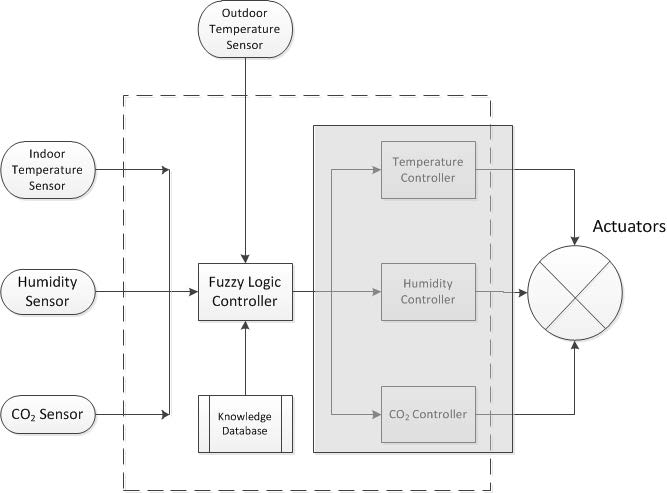
\includegraphics[width=0.85\textwidth]{imgs/arquitectura-FLC.JPG}
	\caption{Arquitectura PID y controlador fuzzy}
	\label{fig:arquitectura-FLC}
\end{figure}

La \autoref{fig:arquitectura-FLC} muestra la arquitectura del FLC, diseñado para regular diferentes variables ambientales mediante un conjunto de sensores y actuadores. Los sensores monitorean parámetros clave, como la temperatura interna y externa, la humedad y la concentración de CO2. Estas lecturas se envían al controlador difuso, que analiza los datos en combinación con una base de conocimiento. Esta base de conocimiento contiene reglas y relaciones definidas por expertos que permiten al sistema tomar decisiones informadas.

El controlador difuso procesa las entradas y determina las acciones necesarias para mantener las condiciones óptimas dentro del entorno. Las decisiones se transmiten a una serie de controladores específicos para cada variable, como el controlador de temperatura, el de humedad y el de CO2. Finalmente, estos controladores ajustan los actuadores correspondientes para implementar las acciones recomendadas. De esta manera, el sistema asegura un ambiente confortable y eficiente, gestionando las interdependencias entre las distintas variables

\vspace{0.4cm}

La \textbf{base de conocimiento} del FLC incluye:
\begin{enumerate}
	\item \textbf{Funciones de membresía}: se utilizan funciones trapezoidales para describir las etiquetas lingüísticas (Bajo, Medio, Alto).
	\begin{figure}[H]
		\centering
		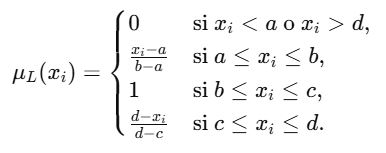
\includegraphics[width=0.55\textwidth]{imgs/function.JPG}
		\caption{Función de membresía}
		\label{fig:function}
	\end{figure}
	
	Se explican algunas variables de la \autoref{fig:function}: $L$ puede tomar el valor de Bajo, Medio y Alto; $a$ y $d$ son los puntos extremos de la función de membresía trapezoidal; $b$ y $c$, los puntos máximos de la función de membresía trapezoidal; y $x_i$ es el $i$-ésimo sensor.
	
	\begin{figure}[H]
		\centering
		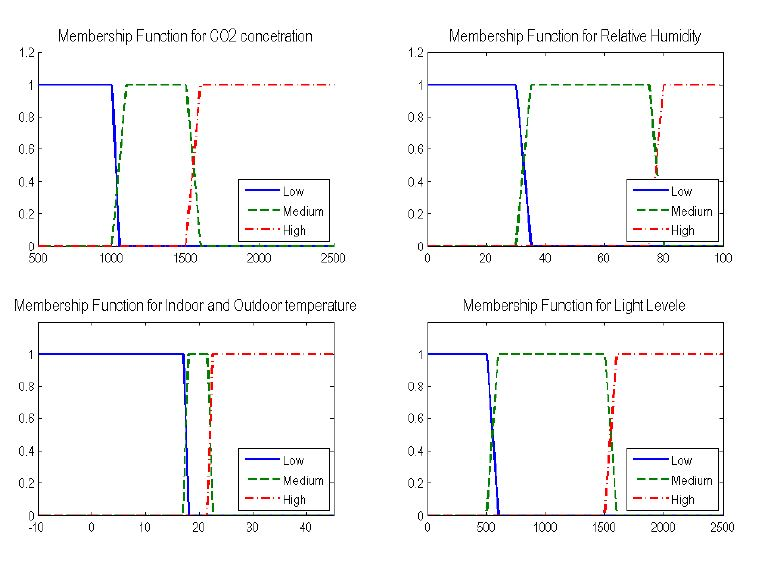
\includegraphics[width=0.8\textwidth]{imgs/membership-functions-input.JPG}
		\caption{Función de membresía de las variables de entrada}
		\label{fig:membership-functions-input}
	\end{figure}
	
	\begin{figure}[H]
		\centering
		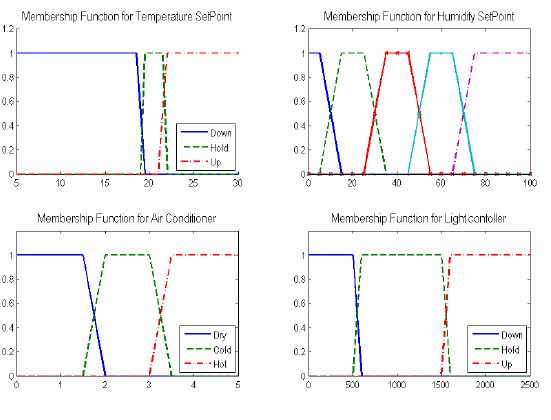
\includegraphics[width=0.8\textwidth]{imgs/membership-functions-output.JPG}
		\caption{Función de membresía de las variables de salida}
		\label{fig:membership-functions-output}
	\end{figure}
	
	\item \textbf{Reglas difusas}: conjunto de reglas IF-THEN derivadas del conocimiento experto. Ejemplos:
	\begin{itemize}
		\item Si la temperatura interna es Media y la externa es Alta, entonces mantener la temperatura y el humidificador en nivel estándar.
		\item Si la humedad es Baja y la temperatura interna es Baja, entonces el aire acondicionado debe estar en caliente, el humidificador en nivel Alto, y subir la temperatura.
	\end{itemize}
	
	Se han utilizado 17 reglas, que dan lugar a diversos escenarios al combinar las posibles entradas del sistema. Se muestra un subconjunto de las reglas en la \autoref{fig:set-of-rules}.
	
	\begin{figure}[H]
		\centering
		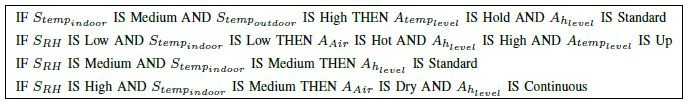
\includegraphics[width=0.9\textwidth]{imgs/set-of-rules.JPG}
		\caption{Conjunto de reglas}
		\label{fig:set-of-rules}
	\end{figure}
	
\end{enumerate}

El motor de inferencia aplica el \textbf{método Mamdani max-min} para combinar reglas y calcular las salidas. Este método evalúa el grado en que cada regla se cumple y combina las salidas difusas.

\begin{figure}[H]
	\centering
	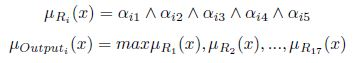
\includegraphics[width=0.55\textwidth]{imgs/mamdani.JPG}
	\caption{Método mamdani max-min}
	\label{fig:mamdani}
\end{figure}

En la \autoref{fig:mamdani}, $x$ son las mediciones de los sensores de entrada, $\alpha_i$ es el grado en que una entrada dada satisface la condición de la $i$-ésima regla ($R_i$), y $\mu_{output_i}$ es la agregación de los conjuntos difusos de salida de todas las reglas para $output_i$.

\subsection{Simulación y pruebas}

\subsubsection{Pruebas con el simulador}

\subsubsection{Pruebas experimentales}

\subsection{Resultados del estudio}
- resumen de resultados

Los resultados obtenidos del estudio indican que el controlador difuso logró mantener las condiciones ambientales dentro de los rangos de confort definidos, con una notable reducción en las fluctuaciones de temperatura y humedad. Durante el período de prueba, el controlador mostró un mejor desempeño que los sistemas reactivos, proporcionando un ambiente más estable y confortable para los ocupantes

- interpretación de los mismos

Estos hallazgos destacan la eficacia del controlador difuso para mejorar la gestión de la calidad ambiental interior. La capacidad del sistema para ajustarse dinámicamente a las condiciones cambiantes del entorno permitió no solo mejorar el confort, sino también optimizar el uso de energía. Esto subraya el potencial de la lógica difusa como una solución integral para sistemas HVAC avanzados en contextos de edificios inteligentes



\newpage
\section{Estudios y enfoques alternativos}

A continuación, se han evaluado dos enfoques alternativos de control difuso de la calidad del ambiente interior, para más adelante hacer un estudio comparativo de los tres.

\subsection{Control fuzzy de sistemas HVAC optimizado con algoritmos genéticos}

Este trabajo, realizado por un investigador de la Universidad de Jaén (Rafael Alcalá) y cuatro de la Universidad de Granada (José M. Benitez, Jorge Casillas, Oscar Cordón y Raúl Pérez) combina control difuso con algoritmos genéticos para optimizar los sistemas HVAC, mejorando la eficiencia energética y el confort \parencite{alcala2003fuzzy}.

El estudio se centró en el control de sistemas HVAC en dos sitios de prueba reales, con el objetivo de optimizar tanto el rendimiento energético como las condiciones de confort interior. Estos sitios incluían un centro de investigación en Francia y una instalación privada. Cada uno tenía características específicas, como sistemas HVAC de diferente configuración, lo que presentaba un desafío adicional para diseñar un controlador adaptable y eficiente. Los expertos proporcionaron modelos térmicos detallados para ambos sitios, ajustados a las condiciones climáticas y de ocupación específicas de cada temporada.

\subsubsection{Diseño del controlador difuso}

El controlador difuso fue diseñado para manejar múltiples criterios, como el confort térmico, la calidad del aire interior y el consumo de energía, usando una base de reglas construida con la experiencia de expertos. Además, se utilizaron funciones de pertenencia triangulares para simplificar el proceso de inferencia y mejorar la manejabilidad del sistema.

A diferencia del estudio principal que se trata en este documento, este proyecto también integró algoritmos genéticos (AG) para afinar automáticamente los parámetros del controlador difuso. Estos AG optimizaron las bases de conocimiento ajustando las funciones de pertenencia para mejorar el rendimiento del sistema bajo diferentes condiciones operativas. El método propuesto recibió el nombre de \textit{Weighted Multi-Criteria Steady-State Genetic Algorithm} (WMC-SSGA), cuyo comportamiento viene reflejado en la \autoref{fig:flowchart-ga}.

\begin{figure}[H]
	\centering
	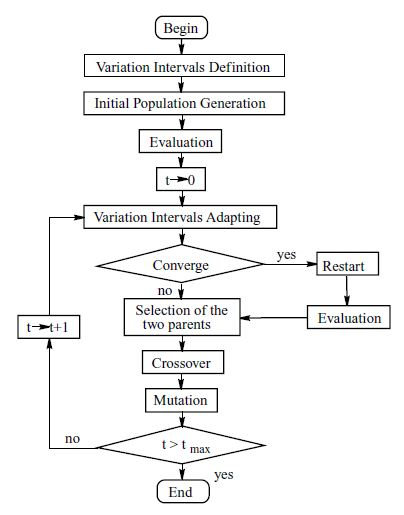
\includegraphics[width=0.45\textwidth]{imgs/flowchart-ga.JPG}
	\caption{Diagrama de flujo del algoritmo WMC-SSGA \parencite{alcala2003fuzzy}.}
	\label{fig:flowchart-ga}
\end{figure}

No se va a entrar en detalle con el funcionamiento del algoritmo genético, pero se podría resumir de la siguiente manera:

El WMC-SSGA comienza con la generación de una población inicial dentro de unos límites. Estas soluciones potenciales codifican parámetros para el controlador difuso, que serán evaluadas por el algoritmo basándose en una función objetivo multicriterio ponderada (con indicadores como minimizar el consumo energético y mantener los niveles de confort). Si no hay suficiente mejora, se ajustan los límites, y después, se seleccionan las mejores soluciones (padres), que se combinan y modifican para crear nuevas soluciones. Este proceso se repite de forma iterativa, evaluando y mejorando las soluciones hasta llegar a un límite o encontrar una solución lo suficientemente buena.

El método anterior contrasta con el FLC unificado, que carece de capacidades de autoajuste y depende únicamente de reglas definidas por expertos.

El controlador difuso presenta una estructura jerárquica, diseñada para procesar múltiples variables y tomar decisiones complejas optimizando el rendimiento del sistema HVAC. Esta estructura se organiza en módulos jerárquicos, donde cada nivel se encarga de tareas específicas y alimenta al siguiente. Se muestra un ejemplo en la \autoref{fig:fuzzy-genetics-functions}.

En la primera capa, se procesan variables básicas como las entradas del índice de control térmico (\textit{PMV}), el valor del PMV anterior (\textit{PMV t-1}), la diferencia entre la temperatura exterior y la interior (\textit{Tout-Tin}) y la posición de la válvula antes del ajuste (\textit{Valve old position}). 

Las flechas entre módulos indican el flujo de la información, señalando cómo los módulos de niveles inferiores sirven para calcular valores que son utilizados como entradas por los niveles superiores. Por ejemplo, partiendo de la \textit{PMV} y \textit{PMV t-1}, se obtiene la preferencia térmica (\textit{Thermal preference}) basada en las condiciones actuales del ambiente. Y esta variable, que pertenece a la segunda capa, puede utilizarse con la \textit{Tout-Tin} para obtener calor requerido (\textit{Required heat}). Este último es necesario en la tercera capa para, junto con la anterior posición de la válvula y la prioridad térmica/energética, poder calcular tanto la nueva posición de la válvula como la velocidad del ventilador del sistema HVAC.

\begin{figure}[H]
	\centering
	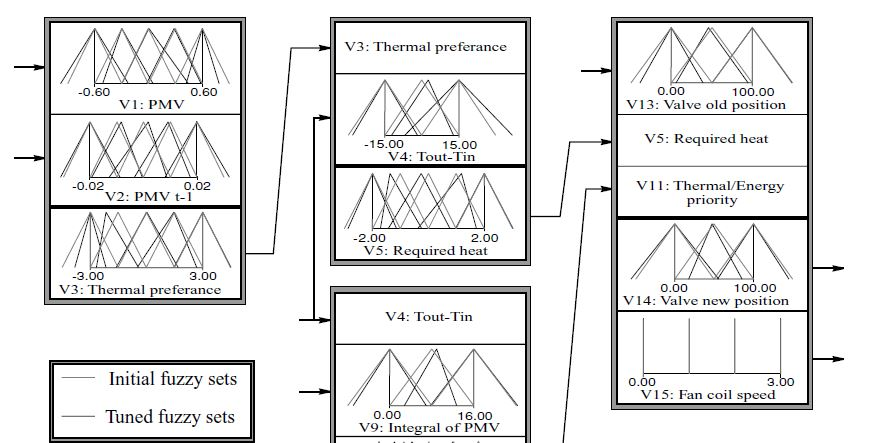
\includegraphics[width=0.95\textwidth]{imgs/fuzzy-genetics-functions.JPG}
	\caption{Diagrama de módulos jerárquicos y funciones de pertenencia \parencite{alcala2003fuzzy}.}
	\label{fig:fuzzy-genetics-functions}
\end{figure}

Las optimizaciones fruto del algoritmo genético vienen reflejadas en la \autoref{fig:fuzzy-genetics-functions} mediante las líneas negras de las gráficas, en contraste con las grises, que representan la configuración original del sistema. Tras la optimización, las funciones muestran ligeros desplazamientos y ajustes en sus picos y bordes, adaptándose mejor a los datos del modelo, ya que estos cambios buscan maximizar la precisión y robustez del sistema.

Asimismo, a diferencia del estudio anterior, en este se ha seguido el \textit{Modo B - FITA} (\textit{First Infer Then Aggregate}). <<En este modo de trabajo, se considera individualmente la contribución de cada conjunto difuso inferido y la acción precisa final se obtiene mediante algún tipo de operación efectuada sobre un valor preciso
característico obtenido a partir de cada conjunto difuso individual. De este modo, se
evita el calculo del conjunto difuso final, lo que ahorra una gran cantidad de
tiempo de cálculo>> \parencite{peregrin2000integracion}. Dicho en otras palabras, cada conjunto difuso resultante de una regla se defuzzifica individualmente, y posteriormente, se utiliza una técnica para combinar los valores crisp obtenidos y así poder producir la salida final.

Para la defuzzificación, en lugar del cálculo del centroide, se ha empleado la técnica \textit{MOM} (\textit{Mean of Maxima}) o media de los máximos, en el que se seleccionan todos los puntos del conjunto difuso de salida donde la función de pertenencia alcanza su valor máximo, para luego calcular el promedio aritmético de esos puntos máximos.

\begin{figure}[H]
	\centering
	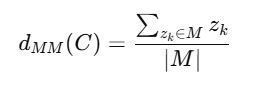
\includegraphics[width=0.33\textwidth]{imgs/mom.JPG}
	\caption{Fórmula de Mean of Maxima (MOM) \parencite{klir1996fuzzy}.}
	\label{fig:mom}
\end{figure}

En la \autoref{fig:mom}, se considera un conjunto $M$ de valores crisp ($z_k$) que tienen el grado de pertenencia máximo dentro del conjunto difuso $C$. 

\subsubsection{Pruebas}

Se llevaron a cabo experimentos tanto en simulaciones como en entornos reales. Los primeros permitieron evaluar durante períodos de 10 días las distintas configuraciones del controlador bajo condiciones climáticas específicas; mientras que los segundos proporcionaron validación en condiciones más realistas. Los resultados se compararon con un controlador convencional On-Off y con versiones iniciales no optimizadas del FLC para medir la mejora alcanzada.

\subsubsection{Resultados y conclusiones}

Al igual que el controlador difuso unificado, los resultados de este estudio mostraron mejoras significativas en comparación con los controladores tradicionales.

En términos de eficiencia energética, en este estudio se lograron ahorros de hasta un 20\% en algunos casos gracias al uso de algoritmos genéticos, mientras que los parámetros de confort se mantuvieron dentro de los rangos deseados con fluctuaciones mínimas. Estos resultados sugieren que la integración de técnicas avanzadas de optimización puede potenciar aún más la eficacia de los controladores difusos.

En comparación con el FLC unificado, este permite la optimización automática de funciones de pertenencia y reglas, logrando un mayor desempeño en el balance entre eficiencia energética y confort, y es altamente escalable para sistemas complejos con múltiples variables y reglas. No obstante, supone una mayor complejidad computacional, su configuración inicial es más costosa y algunos ajusten pueden requerir reentrenamiento con los algoritmos genéticos.

\subsection{Sistema de inferencia difusa centrado en la evaluación de IEQ}

El sistema propuesto por Karol Jabłonski y Tomasz Grychowski, miembros de una universidad polaca, se diseñó para evaluar las condiciones ambientales interiores en un edificio mediante un sistema de sensores y un módulo de inferencia difusa. Similar al primer estudio, este sistema se enfocó en múltiples parámetros como temperatura, humedad y CO2, pero también integró otros factores como iluminación, ruido y olores, proporcionando una evaluación más completa del confort interior \parencite{jablonski2018fuzzy}.

El estudio no describe un controlador difuso en el sentido clásico (es decir, un sistema que toma decisiones para regular un proceso dinámico), sino más bien un sistema de inferencia difusa diseñado para evaluar y calificar el confort ambiental en interiores. Aunque emplea lógica difusa y comparte componentes clave de un controlador difuso (como funciones de pertenencia, reglas difusas y defuzzificación), su propósito es diferente.

Dicho esto, el sistema podría evolucionar hacia un controlador difuso si sus salidas fueran utilizadas para ajustar automáticamente dispositivos como sistemas HVAC.

\subsubsection{Diseño del sistema difuso}

Este estudio adoptó un sistema híbrido de inferencia difusa para procesar múltiples índices, utilizando una estructura modular con subsistemas independientes para manejar los distintos parámetros.

La \autoref{fig:fuzzy-inference-system-diagram} representa el funcionamiento del sistema de inferencia difusa, que se distingue por su enfoque integral, al combinar múltiples parámetros ambientales mediante subsistemas especializados que contribuyen a una evaluación global del confort. 

Las variables monitoreadas incluyen temperatura del aire, temperatura de globo negro, humedad relativa, densidad de CO2, iluminación, ruido y olores, que se procesan a través de módulos de inferencia difusa para estimar diferentes índices de confort. Cada uno de estos índices (confort térmico, frescura del aire y fatiga) es calculado de forma independiente en tres subsistemas, y luego integrado en un módulo principal (confort general) que genera una evaluación global del confort percibido.

Así, a diferencia de los otros dos sistemas que se centran en un conjunto más reducido de variables, este enfoque incluye factores adicionales como olores y ruido, que pueden tener un impacto significativo en la percepción del confort. Además, el sistema consta de 92 reglas difusas, distribuidas entre 4 subsistemas principales, lo que contrasta con un enfoque unificado, que habría requerido hasta 2400 reglas para cubrir todas las combinaciones posibles de entradas.

\begin{figure}[H]
	\centering
	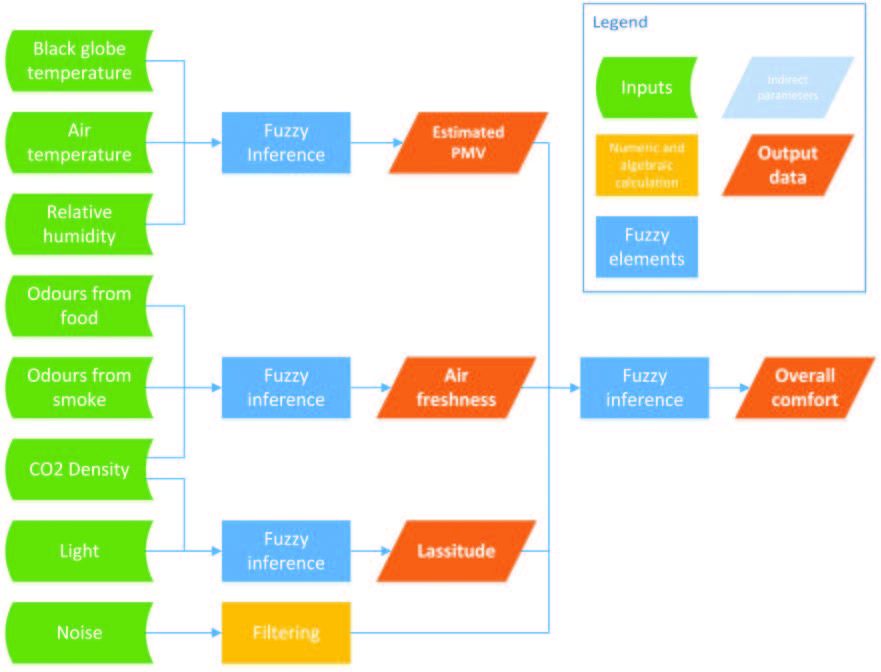
\includegraphics[width=0.75\textwidth]{imgs/fuzzy-inference-system-diagram.JPG}
	\caption{Diagrama del sistema de inferencia difusa \parencite{jablonski2018fuzzy}.}
	\label{fig:fuzzy-inference-system-diagram}
\end{figure}

En este estudio se han utilizado funciones de pertenencia tanto triangulares como trapezoidales, como bien muestra el ejemplo de la \autoref{fig:fis-functions}. 

\begin{figure}[H]
	\centering
	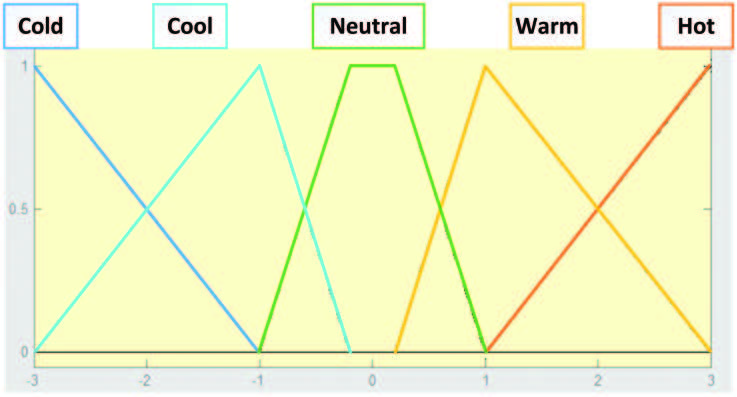
\includegraphics[width=0.5\textwidth]{imgs/fis-functions.JPG}
	\caption{Funciones de pertenencia del confort térmico \parencite{jablonski2018fuzzy}.}
	\label{fig:fis-functions}
\end{figure}

Además, este sistema destaca por implementar un módulo de inferencia en \textit{LabVIEW}, diseñando desde cero los bloques de fuzzificación, inferencia y defuzzificación, mientras que en otros estudios se utilizaron herramientas estándar o adaptaciones de controladores PID.

\subsubsection{Pruebas}

Las pruebas en este sistema se realizaron en un entorno real, con mediciones de confort en diferentes condiciones, incluyendo variaciones en ocupación y ventilación en múltiples escenarios.

Además, lo que le hace destacar del resto es que se tuvieron en cuenta eventos como la presencia de personas o alimentos, en lugar de una habitación cerrada y controlada. La tabla de la \autoref{fig:fis-events} muestra los eventos registrados durante las primeras mediciones del experimento, mientras que las gráficas en la \autoref{fig:fis-output-waveforms} reflejan cómo estos eventos influyen en los índices de confort ambiental, donde subidas en los valores de la tabla indican mayores niveles de alerta o incomodidad.

Por ejemplo, el inicio de una comida en el minuto 22 genera un empeoramiento en la frescura del aire, representada como una leve rampa ascendente en la gráfica, mientras que la apertura de una rejilla de ventilación en la ventana (minuto 182) produce una mejora general en todas las métricas, especialmente en la frescura del aire, lo que tiene sentido ya que permite la renovación del aire del interior.

\begin{figure}[H]
	\centering
	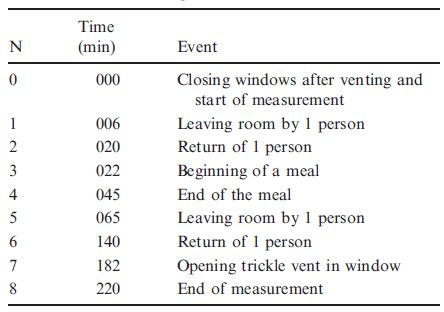
\includegraphics[width=0.7\textwidth]{imgs/fis-events.JPG}
	\caption{Eventos durante las primeras mediciones \parencite{jablonski2018fuzzy}.}
	\label{fig:fis-events}
\end{figure}

\begin{figure}[H]
	\centering
	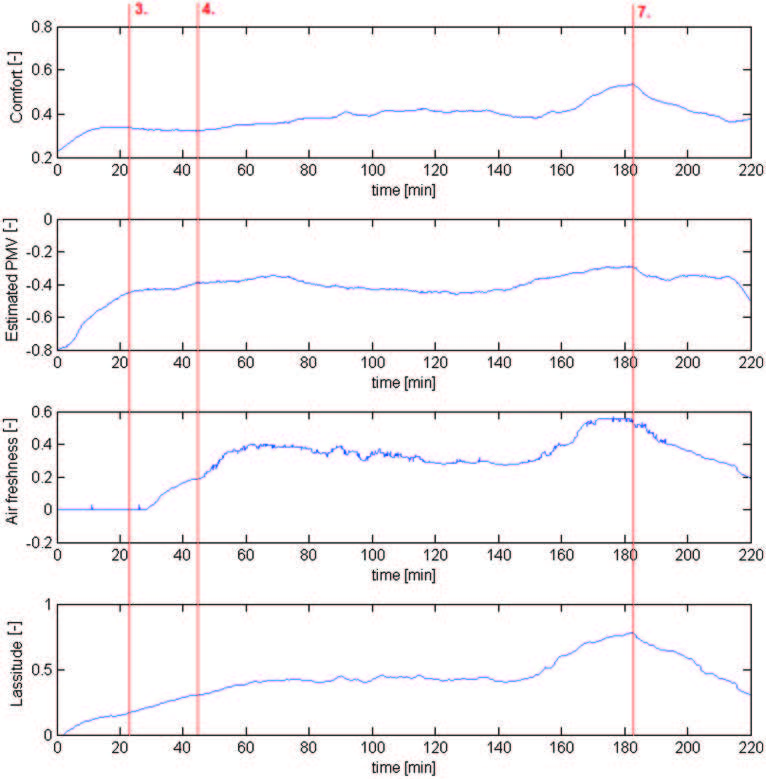
\includegraphics[width=0.7\textwidth]{imgs/fis-output-waveforms.JPG}
	\caption{Formas de onda de los índices de confort \parencite{jablonski2018fuzzy}.}
	\label{fig:fis-output-waveforms}
\end{figure}


Durante las pruebas, se realizaron encuestas para validar los índices calculados por el sistema, permitiendo alinear las percepciones humanas con las salidas del sistema y obteniendo una alta concordancia entre ambas. El enfoque anterior no está presente en los otros dos estudios, donde la validación se centró más en la comparación con sistemas tradicionales o en el análisis de la eficiencia energética.

\subsubsection{Resultados y conclusiones}

En la \autoref{fig:fuzzy-inference-system-results}, se comparan las salidas del sistema difuso con encuestas subjetivas en los cuatro aspectos del confort ambiental definidos por los subsistemas. Los resultados muestran que el sistema sigue tendencias similares a las percepciones humanas, con picos y descensos relacionados con cambios en las condiciones ambientales, aunque es más continuo y menos variable que las encuestas. Esto valida la capacidad del sistema para evaluar objetivamente el confort, reflejando correctamente los efectos de factores como temperatura, iluminación y concentración de CO2.

\begin{figure}[H]
	\centering
	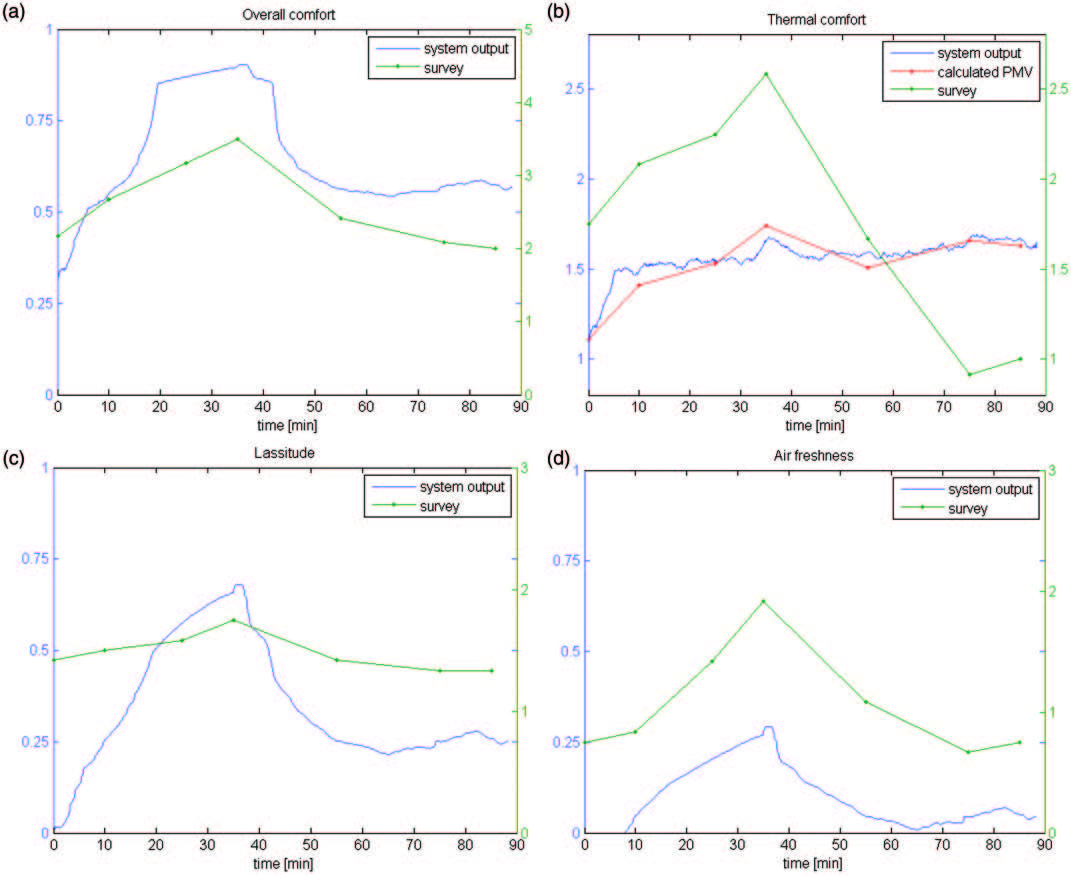
\includegraphics[width=0.76\textwidth]{imgs/fuzzy-inference-system-results.JPG}
	\caption{Resultados de las encuestas y medidas del sistema \parencite{jablonski2018fuzzy}.}
	\label{fig:fuzzy-inference-system-results}
\end{figure}

Este enfoque destaca por la detección de eventos específicos como la presencia de alimentos o cambios en la ocupación. De esta forma, este sistema amplía el rango de variables monitoreadas y evaluadas, proporcionando una evaluación más centrada en todo aquello que define IEQ.

Como ventajas adicionales, Dividir un sistema difuso en subsistemas reduce significativamente la complejidad al evitar el crecimiento exponencial de reglas ($n^m$, siendo $n$ es el número de valores de entrada y $m$ el número de entradas), haciéndolo más manejable y ajustable. La modularidad facilita mejoras y expansiones independientes, como la incorporación de nuevos sensores. Además, mejora la eficiencia computacional al permitir cálculos más simples y rápidas respuestas a cambios ambientales.

Aunque dividir un sistema difuso en subsistemas ofrece claras ventajas, también puede presentar algunas desventajas. Una de ellas es la pérdida de interacción directa entre todas las variables de entrada, lo que puede limitar la precisión en interacciones complejas. También requiere integrar las salidas de los subsistemas, introduciendo incertidumbre o simplificaciones adicionales. Por otro lado, un sistema unificado podría ser más eficiente en hardware potente, ya que procesa todas las combinaciones en una sola etapa.

\subsection{Comparaciones entre los tres estudios}

Las comparaciones entre FLCs diseñados se han realizado en base a cinco aspectos generales:

\begin{table}[H]
	\centering
	\renewcommand{\arraystretch}{1.5}
	\begin{tabular}{|p{2.5cm}|p{4cm}|p{4cm}|p{4cm}|}
		\hline
		\rowcolor{lightgray}
		\textbf{Aspecto} & \textbf{Controlador difuso unificado} & \textbf{Controlador con algoritmos genéticos} & \textbf{Sistema de inferencia difusa} \\ \hline
		
		\textbf{Variables controladas} & 
		Temperatura, humedad, CO2, iluminación & 
		Temperatura, humedad, CO2, consumo energético... & 
		Temperatura, humedad, CO2, iluminación, ruido, olores... \\ \hline
		
		\textbf{Enfoque metodológico} & 
		Controlador difuso clásico con reglas definidas por expertos. FLC supervisa PIDs para HVAC & 
		Integración de algoritmos genéticos para optimizar automáticamente reglas y funciones de pertenencia & 
		Arquitectura modular con subsistemas independientes. Implementación en LabVIEW \\ \hline
		
		\textbf{Pruebas y validación} & 
		Pruebas en una habitación piloto controlada, comparando con controlador reactivo & 
		Simulaciones y pruebas en múltiples entornos reales bajo diferentes condiciones estacionales & 
		Pruebas en entornos ocupados reales, correlacionando resultados con encuestas de usuarios \\ \hline
		
		\textbf{Objetivo principal} & 
		Optimizar el confort interior y la eficiencia energética en sistemas HVAC & 
		Equilibrio dinámico entre confort y eficiencia energética & 
		Evaluación integral del confort interior basado en múltiples índices \\ \hline
		
		\textbf{Aplicación recomendada} & 
		Escenarios con reglas de confort bien definidas, simplicidad y robustez & 
		Entornos donde se requiere máxima eficiencia energética y optimización precisa & 
		Edificios donde la percepción humana del confort es crítica \\ \hline
	\end{tabular}
	\caption{Comparación de tres estudios sobre controladores difusos para IEQ.}
	\label{tab:comparacion}
\end{table}

En conjunto, estos tres enfoques destacan la flexibilidad de los controladores difusos y su capacidad para adaptarse a distintas necesidades y restricciones operativas.

La elección entre estos enfoques dependerá del contexto de aplicación y los objetivos específicos, como si se busca mayor integración en sistemas existentes o una evaluación más detallada de los parámetros de confort.

\newpage
\section{Conclusiones y trabajos futuros}

En conclusión, este

\subsection{Consecución de objetivos}

Se recupera la tabla de objetivos de la sección \textit{1.2.} (Cuadro \ref{tab:subobjetivos}) para marcar aquellos que han sido alcanzados.

\subsection{Trabajos futuros}

Cabe mencionar que la configuración de la habitación experimental descrita en la sección \textbf{\textit{3.3.2.}}, aunque ideal para este tipo de experimentos al permitir un mayor control sobre las variables, no es representativa de un entorno habitado típico. 

En futuros experimentos, se podría introducir factores adicionales, como la presencia de personas y muebles, para evaluar el desempeño del controlador en condiciones más realistas y complejas.



\newpage
\section{Bibliografía}
\defbibheading{empty}{}
\renewcommand{\bibitemsep}{1em}
\printbibliography[heading=empty]

\end{document}